\section{La mise en place d'un cache pour les zones peuplées}
\subsection{Introduction}
Comme nous avons pu le voir dans la partie~\ref{introSolutions}, la mise en place d'un cache pour les zones peuplées permettrait d'améliorer la réactivité dans l'état (\textbf{W}). L'avantage de cette solution, même si l'issue n'était pas certaine, était de s'intéresser à une partie qui n'avait pas encore été étudié dans Blue Banana. Nous avons donc insérer un cache pour chaque nœud de l'environnement, celui-ci va fonctionner dans la continuité de liste des voisins d'un nœud. Nous expliquerons comment nous avons insérer le cache dans le code existant, les différents stratégies que nous avons pu mettre en place et les différents paramètres qui vont influencer le fonctionnent du cache. Nous avons aussi permis l'utilisation du cache pour aider ces nœuds voisins quand ceux-ci cherchent des nœuds.
 
\subsection{Explications de la mise en place du cache}

\subsubsection{Le fonctionnement global et la mise en place du cache dans Blue Banana}
Le fonctionnement global du cache consiste à garder en mémoire un certains nombre de nœuds qui faisait partis de la liste des voisins. Ainsi comme les mouvements de l'avatar sont désordonnés, il est possible qu'il retourne vers des nœuds qu'il vient de quitter. 
\par Sur la figure~\ref{cacheW}, nous pouvons les principales étapes du fonctionnement du cache. Au départ le cache et la liste des voisins sont remplis de différents nœuds. A l'étape 2, le nœud courant (rouge) se déplace et trouve des nouveaux voisins, ceux-ci sont insérés à sa liste des voisins. Deux nœuds sont alors déplacés vers le cache, ce qui pousse deux nœuds hors du cache. A la dernière étape, le nœud courant revient vers une zone qu'il connait, nous détaillerons après le mécanisme de recherche dans le cache, et il trouve deux nœuds dans son cache qui pourraient lui servir pour reconstruire son voisinage. Deux nœuds du cache sont alors insérés dans la liste des voisins du nœud courant, ce qui envoie deux nœuds de cette liste vers le cache. Dans cette exemple, plusieurs nœuds peuvent se déplacer en même temps, ce qui est le cas dans une seul des solutions de cache mise en place.
	\begin{figure}[!h]
        \centering
        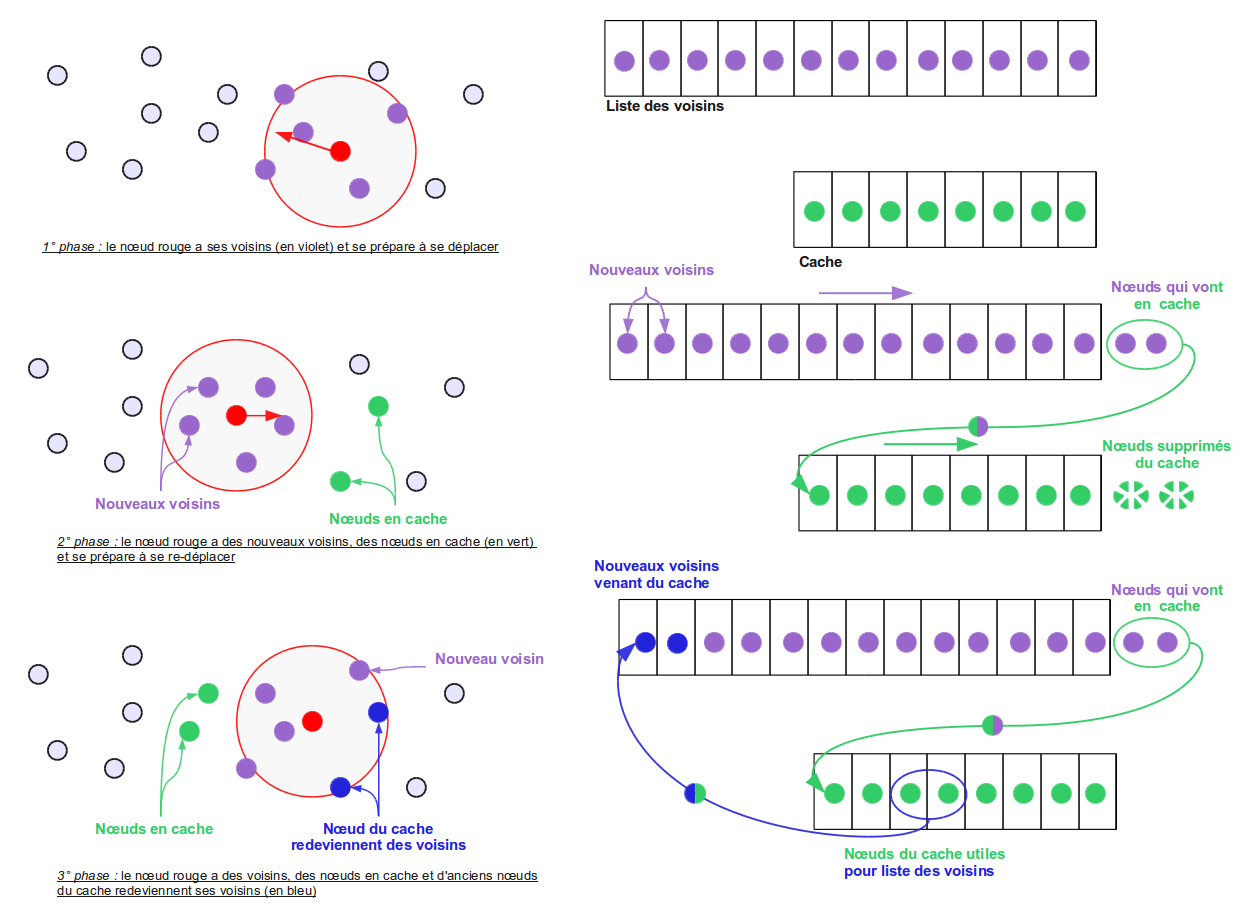
\includegraphics[scale=0.35]{./Ressources/Images/cacheWextends.png}
        \caption{Exemples du fonctionnement global du cache}
        \label{cacheW}
        \end{figure} 
\par Cette solution permet d'économiser des messages de découverte des voisins dans le cas de changements de direction fréquents. Nous verrons dans la partie~\ref{resObesCache} les différents gains et inconvénients de la mise en place du cache. Le cache est donc le prolongement de la liste des voisins pour nœud, mais contrairement à celui-ci , il peut ne pas être tout à fait à jour. Nous avons donc mis en place un système de mis à jour du cache, pour avoir des informations le plus possible exact sur chaque nœud. Mais ce système va coûter cher en nombre de messages, et cela est encore plus vrai plus le cache est grand. Un mécanisme de datation des éléments du cache permet de savoir depuis quand date les informations de chacun. Ce mécanisme nous permet de contacté un nœud pour savoir s'il se trouve toujours à peu près au même endroit, et ainsi l'ajouter ou non à notre voisinage. 

\subsubsection{Les différentes versions du cache}


\subsubsection{L'algorithme de recherche dans le cache}


\subsubsection{La mise en place de l'aide aux voisins grâce au cache}


\subsection{Résultats et observations sur le cache}
\label{resObsCache}

\subsection{Conclusion et perspectives du cache} 



